\documentclass{article}

\usepackage{graphicx}
\usepackage{array}



\begin{document}
	\section{Logic Gates}
	Logic gates perform logical operations that take binary input (0s amd 1s) and produce a single binary output. They are used in most electronic devices including:
	
	\begin{table}[h!]
		\begin{center}
			\caption{Logic Gates}
			\label{tab:table1}
			\begin{tabular}{|l|c|c|}
				\hline
				Smartphones
				&
				Tablets
				&
				Memory Devices
				\\
				\hline
				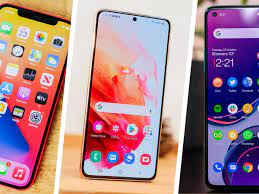
\includegraphics[width=0.2\linewidth]{smartphone}
				
				&
				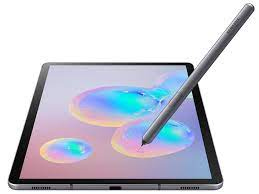
\includegraphics[width=0.25\linewidth]{tablet}
				&
				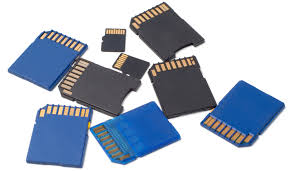
\includegraphics[width=0.2\linewidth]{sd card}
				\\
				 \hline
				 
				 \end{tabular}
		\end{center}
	\end{table}  

\begin{table}[h!]
	\centering\begin{tabular}{| c | m{5cm} | m{5cm} | }
		\hline
		my.github & Advanced & Disadvantages \\ \hline
		\begin{minipage}{.4\textwidth}
			
\includegraphics[width=\linewidth, height=40mm]{github}
			\end{minipage}
		&
		%\begin{minipage}[t]{5cm}
		\begin{itemize}
			\item Easy to contribute to your open source projects
			\item Documentation
			\item Showcase your work \ldots
			\item Track changes in your code across versions
			\item Integration options
			\end{itemize}
		%\end{minipage}
		&
		%\begin{minipage}{5cm}
		\begin{itemize}
			\item Continous integration leads to problems
			\item Not an easy tool for beginners.
			\item Working with larger files can be tricky
			\end{itemize}
		%\end{minipage}
		\\ \hline
		\end{tabular}
	\caption{GitHub Analysis}\label{tbl:mygitHub}
	\end{table}
		
\end{document}